La Work BreakDown Structure, d'ora in poi WBS, rappresenta l'insieme delle attivit\`{a} necessarie a svolgere un compito ben preciso o un processo. Le singole attivit\`{a} prendono il nome di Work Package, WP, e definiscono dettagliatamente le azioni da svolgere per
ciascuna di esse.\\
La WBS \`{e} costituita da una struttura ad albero di WP che, a partire dell'obiettivo finale del progetto, specifica per suddivisioni successive i singoli sotto-obiettivi, fino all'unit\`{a} minima di attivit\`{a}.\\
Tale scomposizione in tanti compiti di dimensioni limitate facilita la gestione, il controllo e l'assegnazione delle singole attivit\`{a}, consentendo una migliore suddivisione del lavoro.\\
Grazie alla WBS il project manager pu\`{o}, in maniera semplificata, organizzare tutte le attivit\`{a} che compongono il progetto, cos\`{i} come i WP, ed avere sempre a disposizione un utile strumento che definisce tutti i passi necessari alla buona realizzazione del progetto.\\
La WBS, inoltre, risulta essere la base per tutte le altre attivit\`{a} di pianificazione richieste per la realizzazione di un progetto di successo.

\begin{figure}[H]
\centering % per centrare l'immagine (opzionale)
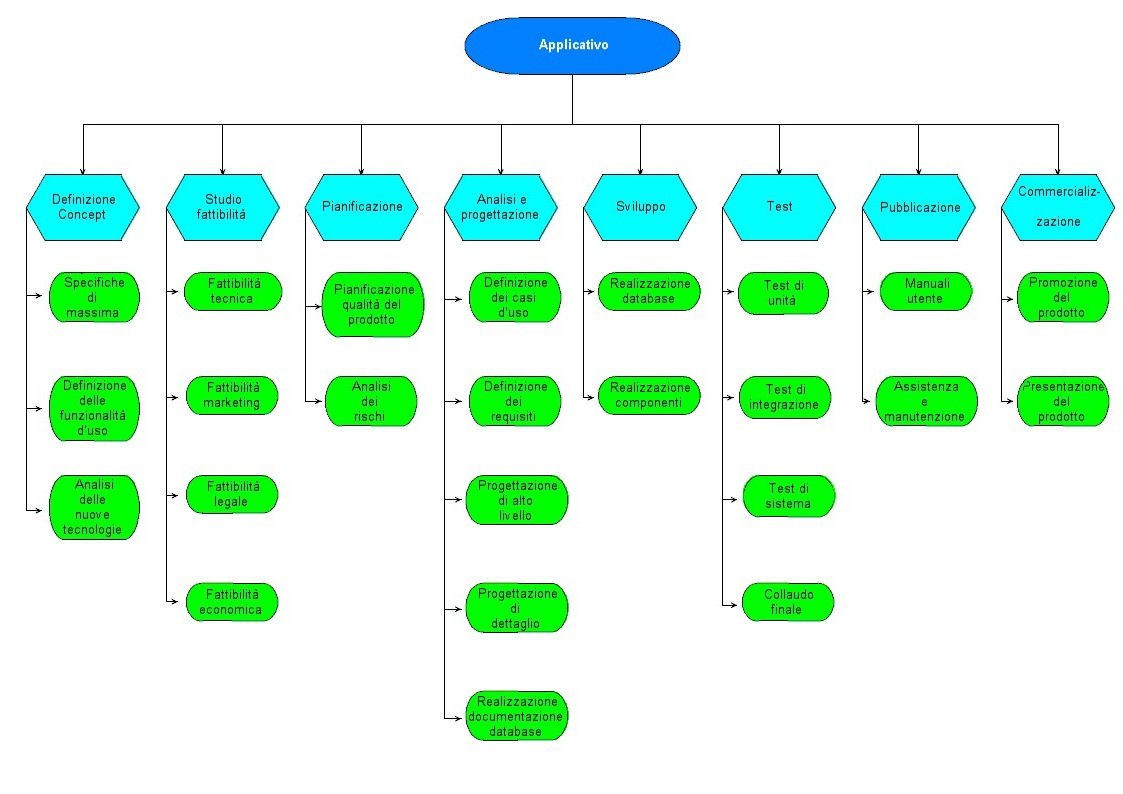
\includegraphics[scale=0.5]{img/Progetto.jpg}
\caption{Diagramma WBS}
\label{fig:Diagramma WBS}
\end{figure}

\subsubsection{WBS-Primo Livello}
\paragraph{Definizione Concept (1.1)}
\`{e} la prima fase del progetto, dove si raccolgono le idee per portare alla nascita e alla definizione del progetto.\\
A partire da questo momento in poi si penser\`{a} alla forma che assumer\`{a} il prodotto finale, alla  definizione delle caratteristiche pi\`{u} importanti (target del prodotto, come si intende erogare il servizio) e alla definizione delle funzionalit\`{a} principali che il prodotto finale deve avere.

\paragraph{Studio Fattibilit\`{a} (1.2)}
\`{e} la fase successiva a quella di Definizione Concept, ha lo scopo di capire se quello che si vuole realizzare \`{e} innanzitutto fattibile e possa portare ad avere dei guadagni concreti.\\
Dunque il concept viene valutato sotto tutti i punti di vista e di interesse per l'organizzazione, al fine di avere un insieme di conclusioni e indicazioni sulle possibilit\`{a} di buona riuscita del lavoro.

\paragraph{Pianificazione (1.3)}
In questa fase si vogliono studiare i processi che il team vuole adottare, quindi una pianificazione delle attivit\`{a} inerenti il ciclo di vita del prodotto avvalendosi di strumenti come diagrammi di Gantt, WBS, OBS e altri strumenti consultabili alla sezione Pianificazione. In questa fase si vogliono definire anche gli obiettivi e le strategie al fine di stabilire a priori ci\`{o} che il team dovr\`{a} controllare e soprattutto misurare.

\paragraph{Analisi e Progettazione (1.4)}
A questo punto gli obiettivi del progetto sono chiari, bisogna dunque formalizzarli e chiarirli in maniera non ambigua.\\
Vengono illustrate dettagliatamente le funzionalit\`{a}, i servizi e le prestazioni che dovranno essere offerte dal prodotto finito.\\
Infine viene progettato come il prodotto soddisfer\`{a} i requisiti definiti in precedenza, definendone la struttura ed architettura da assumere e rispettare.

\paragraph{Sviluppo (1.5)}
In questa fase si passa alla creazione vera e propria del prodotto software mediante la codifica di quanto definito durante la progettazione.\\
Affinché questo risulti possibile \`{e} essenziale che ogni membro si attenga strettamente a quanto descritto nei documenti che gli vengono forniti.\\
Non deve, assolutamente, inserire della creativit\`{a} personale, in quanto il suo compito consiste nella traduzione in codice di quanto deciso precedentemente.\\
Il codice prodotto dovr\`{a} essere costantemente verificato, per avere la sicurezza e la certezza che rispetti i requisiti di qualit\`{a} definiti nella fase di pianificazione, accompagnato dall'appropriata manualistica.

\paragraph{Test (1.6)}
Arrivati a questo punto vengono dunque effettuati i test delle componenti prodotte, verificando come si relazionano tra di loro, a partire dalle componenti di base del prodotto per arrivare a testare, alla fine, il sistema completo.\\
Inoltre viene verificato che quanto \`{e} stato prodotto sia conforme agli obiettivi e ai requisiti che si erano definiti in precedenza.

\paragraph{Post vendita (1.7)}
Una volta che il software prodotto \`{e} terminato e rispetta gli obiettivi ed i requisiti, viene avviato il piano per il rilascio.\\
In questa fase \`{e} prevista la realizzazione di documentazione a supporto dell'utente finale ed eventuali attivit\`{a} di manutenzione o comunque di supporto all'utente finale.\\

\paragraph{Commercializzazione (1.8)}
Questa fase \`{e} stata pianificata al fine di definire come la societ\`{a} intende promuovere il proprio prodotto, ricercare eventuali partnership.

\subsubsection {WBS-Secondo livello}
Per la descrizione dei Work Package di secondo livello verr\`{a} utilizzato il seguente schema in quanto,
, rappresentano tutti insiemi di attivit\`{a} elementari da realizzare:
\begin{description}
\item[Descrizione:] descrizione generica su ci\`{o} che il WP si propone di fare.
\item[Responsabile:] persona che ha la responsabilit\`{a} delle attivit\`{a} da svolgere nel WP e dell'output finale.
\item[Input:] Ci\`{o} di cui necessita in ingresso il WP per iniziare a svolgere le sue attivit\`{a}. Solitamente questi input vengono forniti in uscita da altri WP e possono essere prototipi, documenti o risorse.
\item[Output:] ci\`{o} che il WP deve produrre in uscita. I tipi di uscita possono essere diversi, a seconda delle attivit\`{a} svolte.
\item[Attivit\`{a}:] lista delle attivit\`{a} elementari necessarie al completamento del WP. Per poter essere considerato concluso un WP devono essere concluse tutte le sue attivit\`{a}.
\item[Costo:] costo in euro riassuntivo di tutte le spese necessarie al compimento del WP. Andranno considerate le spese relative al consumo di tutte le risorse utilizzate.
\item[Tempi di realizzazione:] tempo necessario stimato per la buona riuscita e per il completamento del WP, espresso in giorni lavorativi.
\end{description}

\paragraph{Specifiche di massima (1.1.1)}
\begin{description}
\item[Descrizione:] Definizione delle prime specifiche del prodotto per individuare i requisiti ad alto livello necessari a sviluppare l'abstract.
\item[Responsabile:]
\item[Input:] idee, critiche e specifiche provenienti da un brainstorming di gruppo.
\item[Output:] documento formale che descrive una prima versione della specifica del prodotto, nella quale si definisce dettagliatamente l'idea che si vuole realizzare.
\item[Attività:]\mbox{}\\[-1.5\baselineskip]
	\begin{itemize}
	\item ricerca nel web di eventuali competitors per ricavare da progetti gi\`{a} esistenti quali funzionalit\`{a} \`{e} bene riproporre, quali no e quali sono quelle innovative che bisogna sviluppare;
	\item brainstorming tra le risorse umane assegnate al WP per identificare caratteristiche da implementare nel prodotto;
	\item prima stesura documento;
	\item verifica documento ed eventuali correzioni;
	\item formalizzazione documento;
	\item approvazione;
	\end{itemize}
\item[Costo:] 270 \euro{}

\paragraph{Definizione delle funzionalit\`{a} d'uso (1.1.2)}
\begin{description}
\item[Descrizione:] definizione dettagliata delle pi\`{u} importanti funzionalit\`{a} che si vuole siano presenti all'interno del software.
\item[Responsabile:]
\item[Input:] documento di specifiche di massima prodotto dal WP.
\item[Output:] documento che descrive nel dettaglio le funzionalità base che si è deciso di sviluppare.
\item[Attività:]\mbox{}\\[-1.5\baselineskip]
	\begin{itemize}
	\item studio del documento prodotto dal WP;
	\item analisi tecnica di sistemi simili gi\`{a} esistenti;
	\item prima stesura del documento;
	\item verifica del documento ed eventuali correzioni;
	\item formalizzazione del documento;
	\item approvazione.
	\end{itemize}
\item[Costo:] 385 \euro{}
\item[Tempi di realizzazione:] 4 giorni lavorativi.
\end{description}

\paragraph{Analisi delle nuove tecnologie (1.1.3)}
\begin{description}
\item[Descrizione:] ricerca mirata di eventuali innovazioni tecnologie presenti nel mercato che possano risultare utili allo sviluppo del software.
\item[Responsabile:]
\item[Input:] documento di specifiche di funzionalit\`{a} prodotto dal WP.
\item[Output:] documento che descrive nel dettaglio eventuali nuove tecnologie interessanti che potrebbero essere inserite nel progetto. Per ciascuna di queste viene riportata una stima di tempo che si presuppone sia necessario ai programmatori per arrivare ad averne una buona padronanza.
\item[Attività:]\mbox{}\\[-1.5\baselineskip]
	\begin{itemize}
	\item studio del documento prodotto dal WP;
	\item analisi mirata di eventuali nuove tecnologie e stima delle ore per l'apprendimento;
	\item prima stesura documento;
	\item verifica documento ed eventuali correzioni;
	\item formalizzazione documento;
	\item approvazione.
	\end{itemize}
\item[Costo:] 279 \euro{}
\item[Tempi di realizzazione:] 3 giorni lavorativi.
\end{description}

\paragraph{Fattibilit\`{a} tecnica (1.2.1)}
\begin{description}
\item[Descrizione:] fase di valutazione del prodotto che si vuole realizzare dal punto di vista tecnico-tecnologico.
\item[Responsabile:] 
\item[Input:] tutti i documenti prodotti dal secondo livello del WP.
\item[Output:] documento che descrive nel dettaglio, in modo non ambiguo, la fattibilità tecnica per il prodotto che si vuole realizzare indicando le tecnologie e gli strumenti necessari per farlo.
\item[Attività:]\mbox{}\\[-1.5\baselineskip]
	\begin{itemize}
	\item studio dei documenti prodotti dai WP;
	\item incontro fra responsabili i tecnici;
	\item valutazione dei sistemi e degli standard in uso;
	\item valutazione delle tecnologie;
	\item prima stesura documento riassuntivo;
	\item verifica documento ed eventuali correzioni;
	\item formalizzazione documento;
	\item approvazione;
	\end{itemize}
\item[Costo:] 335 \euro{}
\item[Tempi di realizzazione:] 3 giorni lavorativi.
\end{description}

\paragraph{Fattibilit\`{a} marketing (1.2.2)}
\begin{description}
\item[Descrizione:] fase di analisi del mercato per studiare la concorrenza dovuta ad idee similari. Seguono quindi una stima ed una analisi della redditivit\`{a} del prodotto e alle indicazioni preliminari su come pubblicizzarlo e rilasciarlo al fine di ottenere maggiori introiti dalla vendita.
\item[Responsabile:] 
\item[Input:] ricerche di mercato e dati riguardanti eventuali competitor.
\item[Output:] documento formale che indica la fattibilità dal punto di vista del marketing. Nel caso di una buona riuscita sono riportate anche le azioni da seguire per il rilascio del prodotto.
\item[Attività:]\mbox{}\\[-1.5\baselineskip]
	\begin{itemize}
	\item analisi di mercato;
	\item interviste, sondaggi e dialoghi con possibili clienti;
	\item individuazione di eventuali strategie;
	\item prima stesura documento riassuntivo;
	\item verifica documento ed eventuali correzioni;
	\item formalizzazione documento;
	\item approvazione;
	\end{itemize}

\item[Costo:] 319 \euro{}
\item[Tempi di realizzazione:] 3 giorni lavorativi.
\end{description}
\paragraph{Fattibilit\`{a} legale (1.2.3)}
\begin{description}
\item[Descrizione:] fase di analisi del prodotto software sotto l'aspetto legale. Si studiano e si definiscono le strategie eventuali da adottare in difesa del progetto. Si verifica inoltre la possibilit\`{a} di brevettare il prodotto e di registrare un marchio. Infine si verifica che lo sviluppo non porti alla violazione di alcuna legge o normativa in vigore.
\item[Responsabile:]
\item[Input:] conoscenza di eventuali prodotti simili nel mercato e normative/vincoli legali.
\item[Output:] documento formale che indica la fattibilità dal punto di vista legale. Se viene prevista una buona riuscita allora sono riportate anche le azioni da seguire per il corretto rilascio del prodotto.
\item[Attività:]\mbox{}\\[-1.5\baselineskip]
	\begin{itemize}
	\item definizione di un marchio;
	\item consulenza esterna legale;
	\item prima stesura documento riassuntivo;
	\item verifica documento ed eventuali correzioni;
	\item formalizzazione documento;
	\item approvazione;
	\end{itemize}

\item[Costo:] 315 \euro{}
\item[Tempi di realizzazione:] 3 giorni lavorativi.
\end{description}
\paragraph{Fattibilit\`{a} Economica (1.2.4)}
\begin{description}
\item[Descrizione:] fase di analisi del prodotto software sotto l'aspetto economico. Si studia e si valutano i benefici economici che tale progetto potrebbe portare. Vengono stimati inoltre i costi che l'organizzazione dovrebbe sostenere, diretti ed indiretti. Inoltre viene studiata la possibilit\`{a} di ottenere dei finanziamenti esterni 
\item[Responsabile:] 
\item[Input:] conoscenza dei costi diretti ed indiretti delle varie risorse.
\item[Output:] documento formale che indica la fattibilità dal punto di vista economico. All'interno di questo verrà illustrata la previsione economica del prodotto, illustrando i possibili guadagni ed indicando l'eventuale punto di pareggio.
\item[Attività:]\mbox{}\\[-1.5\baselineskip]
	\begin{itemize}
	\item consulenze economiche;
	\item stima dei costi, guadagni e gestione;
	\item ricerca di eventuali finanziatori;
	\item prima stesura documento riassuntivo;
	\item verifica documento ed eventuali correzioni;
	\item formalizzazione documento;
	\item approvazione;
	\end{itemize}
\item[Costo:] 265 \euro{}
\item[Tempi di realizzazione:] 3 giorni lavorativi.
\end{description}

\paragraph{Pianificazione qualit\`{a} del prodotto (1.3.1)}
\begin{description}
\item[Descrizione:] fase di identificazione e definizione degli standard da seguire allo scopo di garantire qualit\`{a} al prodotto. Identificazione delle strategie di controllo da utilizzare per aggiungere qualit\`{a} al prodotto.
\item[Responsabile:] 
\item[Input:] politiche e standard di qualità, esperienze passate degli analisti.
\item[Output:] documenti formali, Piano di Qualifica e Norme di Progetto, che illustrano gli standard e le strategie da seguire per aggiungere qualità al prodotto.
\item[Attività:]\mbox{}\\[-1.5\baselineskip]
	\begin{itemize}
	\item studio degli standard esistenti;
	\item definizione degli obiettivi di qualità;
	\item pianificazione adattamento standard al progetto;
	\item definizione delle strategie di verifica e validazione del software;
	\item definizione delle norme di progetto;
	\item prima stesura documenti riassuntivi;
	\item verifica documenti ed eventuali correzioni;
	\item formalizzazione documenti;
	\item approvazione;
	\end{itemize}
\item[Costo:] 245 \euro{}
\item[Tempi di realizzazione:] 1 giorno lavorativo.
\end{description}

\paragraph{Analisi dei rischi (1.3.2)}
\begin{description}
\item[Descrizione:] fase di analisi dei rischi riguardanti lo sviluppo del prodotto software. Si studia e si definiscono quali sono i rischi in cui si pu\`{o} incombere durante tutte la fasi di sviluppo, cos\`{i} da poterli evitare o quantomeno gestire.
\item[Responsabile:] 
\item[Input:] esperienze personali, conoscenze di rischi noti e documenti prodotti all'interno del WP.
\item[Output:] documento formale che indica gli eventuali rischi che si possono verificare durante le varie fasi di sviluppo del progetto.
\item[Attività:]\mbox{}\\[-1.5\baselineskip]
	\begin{itemize}
	\item identificazione dei rischi noti;
	\item identificazione rischi dovuti alla tipologia del progetto;
	\item ricerca di soluzioni;
	\item prima stesura documento riassuntivo;
	\item verifica documento ed eventuali correzioni;
	\item formalizzazione documento;
	\item approvazione;
	\end{itemize}
\item[Costo:] 255 \euro{}
\item[Tempi di realizzazione:] 2 giorni lavorativi.
\end{description}

\paragraph{Pianificazione del lavoro (1.3.3)}
\begin{description}
\item[Descrizione:] fase in cui viene definita la programmazione delle attivit\`{a} necessarie allo svolgimento del progetto.
\item[Responsabile:] 
\item[Input:] esperienze personali, specifiche di massima, analisi di fattibilit\`{a}.
\item[Output:] WBS,OBS,RBS, diagramma di Gantt.
\item[Attività:]\mbox{}\\[-1.5\baselineskip]
	\begin{itemize}
	\item decisione del livello di profondit\`{a} del WBS;
	\item definizione delle attivit\`{a};
	\item identificazione dei ruoli necessari per lo svolgimento del progetto;
	\item assegnazione dei ruoli alle attivit\`{a};
	\end{itemize}
\item[Costo:] 525 \euro{}
\item[Tempi di realizzazione:] 4 giorni lavorativi.
\end{description}

\paragraph{Definizione dei casi d'uso (1.4.1)}
\begin{description}
\item[Descrizione:]fase di definizione finale delle funzionalit\`{a} del prodotto. Si determina in modo non ambiguo quali saranno le caratteristiche del software e come gli utenti potranno interagire con esso. Successivamente si effettua un'analisi dei rischi sul piano dello sviluppo del software, si studia e si definiscono quali sono i rischi nei quali si pu\`{o} incombere durante tutte la fasi di sviluppo, cos\`{i} da poterli evitare o quantomeno gestire.
\item[Responsabile:] 
\item[Input: ]documentazione prodotta nei WP precedenti ed esperienza personale degli analisti.
\item[Output:] documento formale che illustra chiaramente ed in modo formale le funzionalità definitive del prodotto finale e come sarà possibile per gli utenti interagire con esso.
\item[Attività:]\mbox{}\\[-1.5\baselineskip]
	\begin{itemize}
	\item studio dei documenti in input;
	\item riunione fra gli analisti;
	\item ricerca di soluzioni a problemi emersi durante l'incontro;
	\item prima stesura documento riassuntivo;
	\item verifica documento ed eventuali correzioni;
	\item formalizzazione documento;
	\item approvazione;
	\end{itemize}
\item[Costo:] 445 \euro{}
\item[Tempi di realizzazione:] 4 giorni lavorativi.
\end{description}

\paragraph{Definizione dei requisiti (1.4.2)}
\begin{description}
\item[Descrizione:] fase non elementare, composta da altri WP di livello inferiore, allo scopo di definire i requisiti che il prodotto deve possedere e soddisfare.
\item[Responsabile:] 
\item[Input:] documentazione prodotta nei WP precedenti ed esperienza personale degli analisti.
\item[Output:] documento formale ad uso esterno Analisi dei Requisiti.
\item[Attività:]\mbox{}\\[-1.5\baselineskip]
	\begin{itemize}
	\item studio dei documenti in input;
	\item riunione fra analisti;
	\item prima stesura documento riassuntivo;
	\item verifica documento ed eventuali correzioni;
	\item formalizzazione documento;
	\item approvazione;
	\end{itemize}
\item[Costo:] 821 \euro{}
\item[Tempi di realizzazione:] 6 giorni lavorativi.
\end{description}

\paragraph{Progettazione di alto livello (1.4.3)}
\begin{description}
\item[Descrizione:] fase in cui si procede con la definizione dell'architettura del prodotto utilizzando componenti con
specifica chiara, coesa e nei principi di qualit\`{a} fissati a priori.
\item[Responsabile:] 
\item[Input:] analisi dei requisiti, sistemi aziendali ed eventualmente componenti esistenti.
\item[Output:] documento di specifica tecnica del prodotto che riassume l'architettura generale ed ad
alto livello del software.
\item[Attività:]\mbox{}\\[-1.5\baselineskip]
	\begin{itemize}
	\item incontri tra progettisti e analisti;
	\item analisi di componenti e sistemi esistenti;
	\item valutazione di essi per opportunità di riuso;
	\item identificazione componenti fondamentali;
	\item individuare le tecnologie e le tecniche da utilizzare;
	\item prima bozza di documenti e schemi, revisione, approvazione, formalizzazione finale.
	\end{itemize}
\item[Costo:] 976 \euro{}
\item[Tempi di realizzazione:] 4 giorni lavorativi.
\end{description}

\paragraph{Progettazione di dettaglio (1.4.4)}
\begin{description}
\item[Descrizione:] fase in cui si procede con la definizionedelle unit\`{a} realizzative cio\`{e} moduli la cui complessit\`{a} deve essere ridotta al minimo indispensabile al fine di permettere la realizzazione del modulo al singolo programmatore.
\item[Responsabile:] 
\item[Input:] analisi dei requisiti, specifica tecnica.
\item[Output:] documento di definizione del prodotto che descriva con linguaggio UML2.0 schemi e diagrammi di tutte le unità che devono essere realizzate.
\item[Attività:]\mbox{}\\[-1.5\baselineskip]
	\begin{itemize}
	\item definizione e specifica dei moduli da realizzare
	\item raggruppare moduli in unità mantenendo basso accoppiamento e elevata coesione
	\item assegnare le unità ai componenti
	\item tracciamento componenti- requisiti
	\item stabilire i test di unità
	\item prima stesura del documento, revisione, approvazione, formalizzazione finale.
	\end{itemize}
\item[Costo:] 1405 \euro{}
\item[Tempi di realizzazione:] 10 giorni lavorativi.
\end{description}

\paragraph{Documentazione database (1.4.5)}
\begin{description}
\item[Descrizione:] stesura formale della documentazione relativa all'architettura riguardante il database.
\item[Responsabile:] 
\item[Input:] specifica tecnica, definizione di prodotto.
\item[Output:] documento con scopo documentale della codifica del software.
\item[Attività:]\mbox{}\\[-1.5\baselineskip]
	\begin{itemize}
	\item studio documenti in input;
	\item stesura documentazione per ogni singola unità;
	\item verifica documento ed eventuali correzioni;
	\item formalizzazione documento;
	\item approvazione;
	\end{itemize}
\item[Costo:] 355 \euro{}
\item[Tempi di realizzazione:] 2 giorni lavorativi.
\end{description}

\paragraph{Realizzazione database (1.5.1)}
\begin{description}
\item[Descrizione:] fase di sviluppo e codifica del database secondo quanto definito nella fase di progettazione.
\item[Responsabile:] 
\item[Input:] Analisi Requisiti, Specifica Tecnica, Definizione di Prodotto, Norme di Progetto, Piano di Qualifica ed altra documentazione tecnica.
\item[Output:]database realizzato e pienamente funzionante.
\item[Attività:]\mbox{}\\[-1.5\baselineskip]
	\begin{itemize}
	\item studio dei documenti in input;
	\item fase di codifica;
	\item verifica del codice e delle funzionalit\`{a} del database;
	\item verifica della qualit\`{a};
	\item approvazione;
	\end{itemize}
\item[Costo:] 575 \euro{}
\item[Tempi di realizzazione:] 5 giorni lavorativi.
\end{description}

\paragraph{Realizzazione componenti (1.5.2)}
\begin{description}
\item[Descrizione:] fase di sviluppo e codifica delle componenti previste nella fase di progettazione comprensive sia dell'interfaccia grafica del prodotto, sia delle logica dell'applicativo.
\item[Responsabile:] 
\item[Input:] Analisi Requisiti, Specifica Tecnica, Definizione di Prodotto, Norme di Progetto, Piano di Qualifica ed altra documentazione tecnica.
\item[Output:] codice dell'applicativo.
\item[Attività:]\mbox{}\\[-1.5\baselineskip]
	\begin{itemize}
	\item studio dei documenti in input;
	\item fase di codifica;
	\item verifica del codice;
	\item verifica della qualit\`{a};
	\item approvazione;
	\end{itemize}
\item[Costo:] 6755 \euro{}
\item[Tempi di realizzazione:] 21 giorni lavorativi.
\end{description}

\paragraph{Test di unit\`{a} (1.6.1)}
\begin{description}
\item[Descrizione:] fase di test di tutte le singole unit\`{a} software prodotte.
\item[Responsabile:] 
\item[Input:] metodi pianificati nell'architettura di dettaglio del prodotto.
\item[Output:] documento riassuntivo dei risultati ottenuti dai test.
\item[Attività:]\mbox{}\\[-1.5\baselineskip]
	\begin{itemize}
	\item studio documento in input;
	\item esecuzione dei test;
	\item risoluzione eventuali errori rilevati;
	\item approvazione dei test;
	\item stesura documento riassuntivo;
	\item verifica documento;
	\item formalizzazione documento;
	\item approvazione;
	\end{itemize}
\item[Costo:] 990 \euro{}
\item[Tempi di realizzazione:] 21 giorni lavorativi.
\end{description}

\paragraph{Test di integrazione (1.6.2)}
\begin{description}
\item[Descrizione:] fase di test delle singole funzionalit\`{a} del prodotto, si tratta di una verifica in primis dei flussi di dati in entrata e in uscita tra le varie componenti realizzate e infine nella verifica dei flusso di controllo tra le componenti.
\item[Responsabile:] 
\item[Input:] componenti pianificati nella specifica tecnica del prodotto (progettazione di alto livello).
\item[Output:] documento riassuntivo dei risultati ottenuti dalla batteria di test realizzati.
\item[Attività:]\mbox{}\\[-1.5\baselineskip]
	\begin{itemize}
	\item studio documento in input;
	\item esecuzione dei test;
	\item risoluzione eventuali errori rilevati;
	\item approvazione dei test;
	\item stesura documento riassuntivo;
	\item verifica documento;
	\item formalizzazione documento;
	\item approvazione;
	\end{itemize}
\item[Costo:] 1080 \euro{}
\item[Tempi di realizzazione:] 20 giorni lavorativi.
\end{description}

\paragraph{Test di sistema (1.6.3)}  
\begin{description}
\item[Descrizione:] fase di test sulle interazioni fra le singole unit\`{a}. Si verifica che i comportamenti in seguito alle comunicazioni fra di queste siano quelli previsti. Queste fase ha lo scopo principale di effettuare un collaudo interno al fine di compiere eventuali correzioni onde evitare malfunzionamenti per il collaudo finale del prodotto.
\item[Responsabile:] 
\item[Input:] interfaccia grafica e Piano di Qualifica, documento riassuntivo test di unit\`{a}.
\item[Output:] documento riassuntivo dei risultati ottenuti dai test di integrazione.
\item[Tempi di realizzazione:] 2 giorni lavorativi.
\end{description}

\paragraph{Collaudo finale (1.6.4)}
\begin{description}
\item[Descrizione:] fase di test dell'intero sistema da effettuare prima del rilascio. Si cercano eventuali errori o malfunzionamenti e successivamente si certifica che tutte le funzionalit\`{a} dichiarate siano presenti.
\item[Responsabile:] 
\item[Input:] interfaccia grafica, esito dei vari test, Piano di Qualifica e Analisi Dei Requisiti.
\item[Output:] documento riassuntivo dei risultati ottenuti dai test e dal controllo dei requisiti.
\item[Attività:]\mbox{}\\[-1.5\baselineskip]
	\begin{itemize}
	\item studio documenti in input;
	\item esecuzione di test di sistema previo utilizzo;
	\item risoluzione eventuali errori rilevati;
	\item approvazione dei test;
	\item controllo dei requisiti soddisfatti;
	\item stesura documento riassuntivo;
	\item verifica documento;
	\item formalizzazione documento;
	\item approvazione;
	\end{itemize}
\item[Costo:] 315 \euro{}
\item[Tempi di realizzazione:] 1 giorno lavorativo.
\end{description}

\paragraph{Manuali Utente (1.7.1)}
\begin{description}
\item[Descrizione:] realizzazione dei manuali utente per il supporto all'utente all'uso dell'interfaccia. Il manuale illustra le funzionalit\`{a} del prodotto, il suo utilizzo e l'esposizione di problemi con le possibili soluzioni.
\item[Responsabile:] 
\item[Input:] interfaccia prodotto.
\item[Output:] documento con lo scopo di fornire un supporto agli utenti dopo il rilascio.
\item[Attività:]\mbox{}\\[-1.5\baselineskip]
	\begin{itemize}
	\item studio delle funzionalit\`{a} del software;
	\item prima realizzazione manuale;
	\item verifica documento ed eventuali correzioni;
	\item formalizzazione documento;
	\item approvazione;
	\end{itemize}
\item[Costo:] 525 \euro{}
\item[Tempi di realizzazione:] 4 giorni lavorativi.
\end{description}

\paragraph{Assistenza e manutenzione (1.7.2)}
\begin{description}
\item[Descrizione:] fase che segue il rilascio del software: in questa fase bisogna prevedere
possibili bug del prodotto e problemi che si possono verificare con i clienti e che dovranno essere risolti.
\item[Responsabile:] 
\item[Input:] problema riguardante il software.
\item[Output:] rilascio nuova versione, relazioni sui problemi incontrati e sulle soluzioni,
\item[Attività:]\mbox{}\\[-1.5\baselineskip]
	\begin{itemize}
	\item il servizio clienti \`{e} in contatto con il cliente per rilevare la
	soddisfazione del prodotto tramite interviste e questionari per fornire assistenza;
	\item progettisti e programmatori lavorano per risolvere eventuali problemi individuati;
	\end{itemize}
\item[Costo:] 3610 \euro{}
\item[Tempi di realizzazione:] 47 giorni lavorativi.
\end{description}

\paragraph{Promozione del prodotto (1.8.1)}
\begin{description}
\item[Descrizione:] fase di promozione del prodotto realizzato. Si punta a pubblicizzare il prodotto con lo scopo di raggiungere quanti pi\`{u} clienti possibili iniziando a creare un brand.
\item[Responsabile:] 
\item[Input:] alcune conoscenze di marketing e target clienti.
\item[Output:] slogan, pubblicità scelte di mercato da intraprendere.
\item[Attività:]\mbox{}\\[-1.5\baselineskip]
	\begin{itemize}
	\item ricerca possibili clienti;
	\item pubblicità rivolta alla categorie di clienti scelti;
	\end{itemize}
\item[Costo:] 730 \euro{}
\item[Tempi di realizzazione:] 11 giorni lavorativi.
\end{description}

\paragraph{Presentazione del prodotto (1.8.2)}
\begin{description}
\item[Descrizione:] il prodotto software verr\`{a} presentato in opportuni incontri con dei potenziali clienti al fine di dimostrare l'utilit\`{a} del prodotto.
\item[Responsabile:] 
\item[Input:] software completato.
\item[Output:] incremento delle conoscenze del prodotto stesso e del team a possibili acquirenti e investitori. 
\item[Attività:]\mbox{}\\[-1.5\baselineskip]
	\begin{itemize}
	\item dimostrazione dell'utilit\`{a} del prodotto;
	\item raccolta feedback.
	\end{itemize}
\item[Costo:] 315 \euro{}
\item[Tempi di realizzazione:] 1 giorno lavorativo.
\end{description}
